
\section{Theory}
\label{sec:theory}
\subsection{Load Path}
A floating wind turbine undergoes loading from a number of sources.
Some of these loads are calculated within \textit{FloatingSE} and some are
calculated in other WISDEM modules.  Wind and wave loads are computed
here.  Rotor thrust loads are computed in \textit{RotorSE}, and imputed into
\textit{FloatingSE} as inputs.  All loading, including gravity loads, over the
entire turbine are assembled within \textit{FloatinSE} for a structural analysis
via Frame3DD.  Once all member loads and stresses are determined,
compliance checks against international standards are evaluated and can
be used as design constraints during optimization runs.

\subsubsection{Wind and Wave Loads}
Wind drag loads are applied to the tower body and the upper part of the
substructure that extends above the waterline.  These drag loads are
computed assuming the tower and columns are smooth circular
cross-sections and that the drag coefficient can be selected as a
function of the flow Reynolds number \citep{Roshko}.  The drag, Reynolds
number (and drag coefficient) are allowed to vary as a function of
height, according to the wind velocity distribution selected by the user
(power-law or logarithmic variation),
\[
Re_d = \frac{\rho_a U(z) d(z)}{\mu_a},\qquad dF(z) = \frac{1}{2} \rho U^2(z)
d(z) c_d(Re) dz
\]
where $\rho_w$ and $\mu_w$ are the density and viscosity of air, $U(z)$
is the velocity as a function of height, $d(z)$ is the diameter of the
body as a function of height, $c_d$ is the drag coefficient, and $dF(z)$
is the force per unit length in the z-direction.. All of the
calculations necessary for wind drag loading are found within the WISDEM
\textit{CommonSE} module, with separate OpenMDAO Components for the velocity
profile and the drag forces.

Wave drag loads are computed using Morison's equation.  Morison's
equation is a semi-empirical expression, as opposed to a
model of a specific physical process, that predicts the total
hydrodynamic loads.  It is comprised of two components, one for viscous
drag contributions and another for inertial effects (which includes incident,
diffracted, and radiated wave effects),
\begin{equation} \label{eqn:morison}
  dF(z) = \frac{\pi d^2(z)}{4} \rho C_m \dot{U}(z)dz + \frac{1}{2} \rho U^2(z) d(z) c_d(Re)dz
\end{equation}
where $C_m$ is the added mass coefficient (assumed to be $C_m=2$),
$U(z)$ is the current speed as a function of height, and
$\dot{U}$ is the acceleration of the current.

The calculations of the wind and wave loads are separated from the
actual velocity distributions within \textit{CommonSE}.  The wind and wave
velocities are handled by the \textit{CommonSE} \texttt{environment} module,
where wind profiles can assume a power-law or logarithmic shape (given a
reference height and velocity) and wave profiles are derived from linear
(Airy) wave theory (given a significant wave height and periodicity).

\subsubsection{Structural Analysis}
The whole floating turbine load path, from the rotor to the keel of the
substructure, is modeled with a simple frame element tool.  The forces,
moments, and mass properties of the rotor-nacelle assembly (RNA) are
inputs to \textit{FloatingSE} (mass properties are assumed to be relative to the
tower top position).  It is also assumed that the RNA is a rigid body
with respect to the tower modes.  Long slender components, such as the
tower and substructure columns, can be broken up into a finer
discretization than the physical ``cans'' that they are actually made
of.  This finer discretization gives greater resolution of internal
forces and natural frequencies.  Substructure pontoons are represented
as single frame elements.  Rigid boundary conditions for all 6 degrees
of freedom (DOF) are imposed at the windward mooring line connection,
which is assumed to be aligned with the wind, wave, and rotor thrust
loads.  Aside from the RNA loads, other loads applied to the structure
include the wind and wave forces described above, the gravity loads, and
the buoyancy acting on the submerged elements.

Frame elements are described by their cross sectional properties (area,
moments of inertia, modulus of elasticity, and mass density) and
starting and ending nodes.  For simple geometries, such as pontoons with
tubular cross sections, these properties are straightforward
calculations.  For the turbine tower, tubular cross section properties
are also used, albeit at a finer discretization.  For substructure
columns, which may have permanent or variable ballast and bulkheads,
it is assumed that they extra components are not load-bearing, so
tubular cross section properties are also used.  However, the material mass
density of the frame element is scaled to reflect the true mass of the
whole section, including ballast, to ensure that gravity loads are
captured correctly.

Simulation outputs include mass properties of the structure, member
stresses, and summary forces and moments on the body.  Mass properties
include the total mass of the floating turbine and the mass of the
substructure itself.  The calculations also allow for easy computation
of the center of mass of the structure, not accounting for variable
ballast which is computed elsewhere, and the center of buoyancy
(centroid of the submerged volume).  The first two natural frequencies
of the structure are also computed to compare against the rotor passing
frequencies (1P and 3P).  Next, the reaction forces and moments at the
boundary mooring load are taken as the total loading on the structure.
These are used later in the static stability calculations to ensure that
the mooring lines provide adequate restoring force and moment.  Finally,
the axial and shear forces  are extracted and converted
to stresses using cross-section properties for all elements.  Hoop
stress of the tower is estimated from the dynamic pressure head of the
wind loads using the Eurocode method.  Hoop stress of the submerged
columns is determined using the dynamic and static pressure heads of the
water.  All stress components are combined into a von Mises stress for
comparison against a yield criterion.

The analysis tool, Frame3DD, is an open-source tool for static and
dynamic structural analysis of 2-D and 3-D frames and trusses with
elastic and geometric stiffness. It computes the static deflections,
reactions, internal element forces, natural frequencies, and modal
shapes using direct stiffness and mass assembly \citep{frame3dd}.  The
WISDEM toolkit developed a python interface, \textit{pyFrame3DD}, to avoid the
use of intermediate input and output text files.

Much of the numerical technique used by Frame3DD relies on entry of
cross sectional properties for all of the elements.  For the tower,
columns, and pontoons, only cylindrical (tubular) cross-sections are
supported for now.  Future development may support other cross-sectional
geometries.  For the tubular cross, the critical properties needed by
Frame3DD are,
\begin{align*}
  \textrm{Outer radius, } r_o &= d/2\\
  \textrm{Inner radius, } r_i &= r_o - t\\
  \textrm{Material area, } A &= \pi \left( r_o^2 - r_i^2 \right)\\
  \textrm{Bending second moment of area, } I_{xx} &= I_{yy} = \frac{\pi}{4}\left( r_o^4 - r_i^4 \right)\\
  \textrm{Torsion second moment of area, } I_{zz} &= J_0 = I_{xx} + I_{yy}\\
  \textrm{Shear area, } A_{sx} &= A_{sy} = A / \left[ 1.124235 +
           0.055610\left(\frac{r_i}{r_o}\right) +
           1.097134\left(\frac{r_i}{r_o}\right)^2 - 0.630057\left(\frac{r_i}{r_o}\right)^3 \right]\\
  \textrm{Bending modulus, } S &= I_{xx} / r_o \\
  \textrm{Torsion modulus (shear constant), } C &= I_{zz} / r_o \\
\end{align*}
where $d$ is the tube diameter and $t$ is the tube (or wall) thickness,
which are the common design variables for the tower, columns, and
pontoons. Note that the shear area expression is an empirical relationship as
opposed to an analytical expression.

\subsubsection{Code Compliance}
Once the stress components of all structural members are computed, they
are compared against accepted design code standards for compliance.
These standards serve as design constraints when conducting optimizing.

Differing code standards are used for different components.  The turbine
tower and substructure pontoons stress components (axial, shear, and
hoop) are evaluated against a von Mises yield criterion with an
allowance for a margin of safety.  Tower segment stresses and geometry
are also evaluated against a shell buckling criterion published by
Eurocode \citet{Eurocode} and a global buckling criterion Germanischer
Lloyd \citet{Germanischer}.  Note that the implementation of the
Eurocode buckling is modified slightly so as to produce continuously
differentiable output. Since the tower is typically reinforced at
shorter distances than the full tower length, the user may specify the
reinforcement length.

The buckling criterion applied to the tower are not suitable for the
submerged columns of a spar or semisubmersible substructure due to the
higher hydrostatic pressure loads and use of ring stiffeners.  For these
submerged columns, the code standards applied are from the American
Petroleum Institute, Bulletin 2U \citep{api2U} (specifically the
procedure outlined in Appendix B).  These standards also apply shell and
general buckling criterion with a margin of safety.


\subsection{Static Stability}
\label{sec:static}
\subsubsection{Neutral Buoyancy}
Any floating body requires enough water displacement to create
sufficient buoyancy force such that the body stays afloat in the most
extreme loading and environmental conditions.  This level of
displacement would then otherwise be overkill for more benign loading
conditions.  Since a floating turbine is designed for a constant hub
height, variable amounts of ballast are required to maintain a neutrally
buoyant system for all operating conditions.  The variable ballast is
simply ocean water that is pulled in or pumped out of holding areas
within the substructure columns.

In \textit{FloatingSE}, the variable ballast water mass is calculated as the
difference between the total mass of displaced water and the total mass
of the floating turbine.  This mass is then divided by the water density
to obtain the variable ballast volume, which is then compared to the
frustum shell cross section profile above the permanent ballast to
determine the height of the water ballast within the column.  Once this
is determined, the final center of mass and center of buoyancy (centroid
of the submerged volume) of the
system can be determined.

\subsubsection{Surge/Sway Stability}
Surge and sway stability is not actively tracked over the coarse of a
load case.  Instead the total surge force on the structure is calculated
and compared to the restoring force of the mooring system at the maximum
allowable surge offset, which is specified by the user.  If the
restoring force at this maximum offset is greater than the surge force
applied, then the system is considered stable in surge.  Since the wind
and wave profiles are essentially 2-D in the $x-z$ plane, there are no
sway forces or motions at play.  Thus, sway stability is given the same
status as surge stability.

The surge direction is assumed to be aligned with the wind vector, which
is aligned with the $x$-axis.  Since the rotor yaw is assumed to be
$0^{\circ}$, the surge forces on the turbine include the rotor thrust,
the wind drag on the tower, and the wind and wave drag on the
substructure.  The final surge force over the whole structure is taken
from the $x$-direction reaction force of the windward reaction node in
the turbine-level Frame3DD analysis.  The total surge force applied is
only calculated at the zero-displacement point, and not at the maximum
offset condition.

The restoring force is calculated as the smallest possible restoring
force after a displacement in any angular direction.  Since the
alignment of the mooring lines relative to the incoming wind direction
is arbitrary, a maximum offset is simulated at $2^{\circ}$ increments
around the circle.  The smallest restoring force is used for the surge
stability calculations.  Also recorded is the maximum mooring line
tension in any direction, for comparison against the minimum breaking
load value.

\subsubsection{Pitch Stability}
The approach to pitch stability determination is similar to that of
surge stability.  The total pitching moment on the floating turbine is
calculated and compared to the restoring moment at the maximum allowable
angle of heel.  If the restoring moment at this max heel angle is
greater than the pitching moment applied, the system is said to be
statically stable in pitch.

Similar to the surge force calculation, the total pitching moment is
determined from the reaction moment at the windward boundary condition
in the Frame3DD analysis.  The pitching moment has contributions from
the wind and wave loads on the structure, the rotor forces and torques,
the buoyancy forces on the submerged substructure, and the off-center
weight of components (e.g. the RNA).  The total pitching moment is only
calculated at the $0^{\circ}$ pitch point, and not at the maximum heel
angle condition.

The restoring pitching moment has two primary contributions.  The first
is from the mooring lines.  Similar to the surge force calculation, here
the floating turbine is deflected in pitch by the maximum allowable heel
angle and the mooring forces are recorded.  Within the mooring
calculation, the center of mass of the turbine is not known, but these
forces are saved in the simulation until that point is computed.  Then,
the restoring moment contribution from the mooring system is computed as,
\[
  \mbf{M_{moor}} = \sum_i \mbf{r_{cm-i}} \times \mbf{F_i}
\]
where $r_{cm-i}$ is the vector from the center of mass to the mooring
connection, $i$, and $F_i$ is the force applied by the $i$\th mooring
line.
\begin{figure}
  \begin{subfigure}[b]{0.49\linewidth}
    \centering 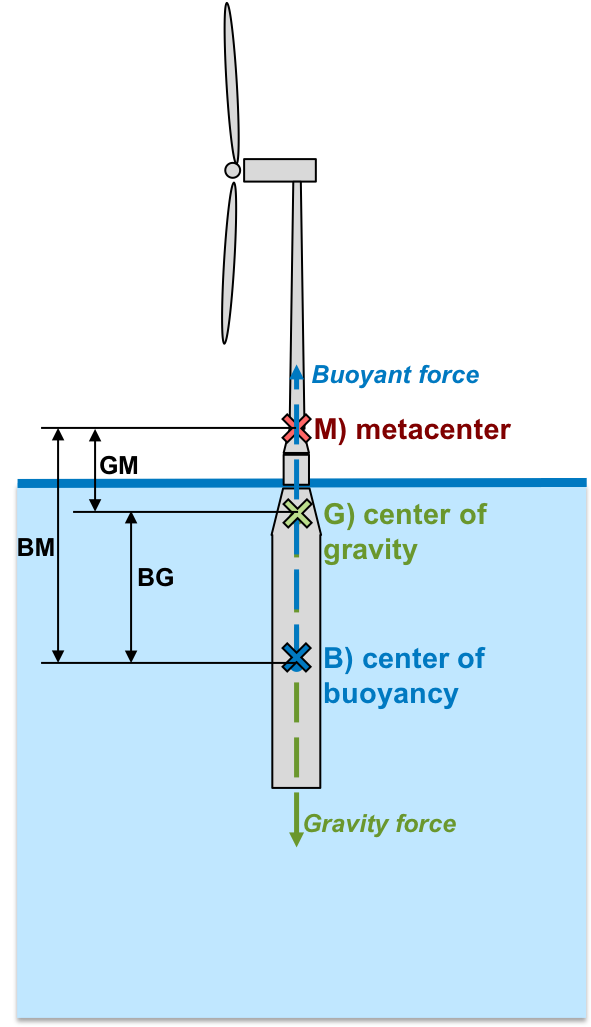
\includegraphics[height=3.5in]{figs/metacenterA}
    \caption{}
  \end{subfigure}
  \begin{subfigure}[b]{0.49\linewidth}
    \centering 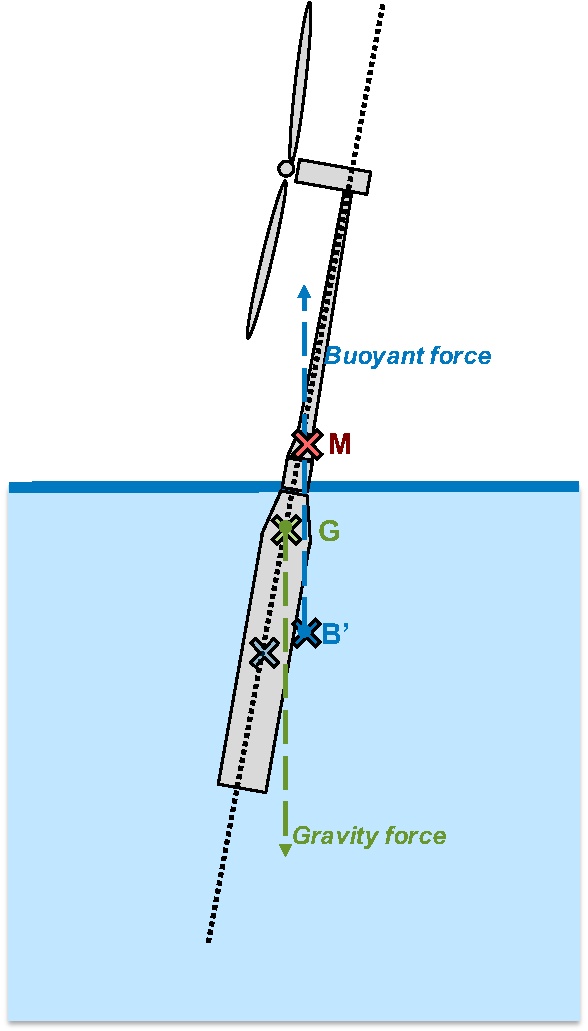
\includegraphics[height=3.5in]{figs/metacenterB}
    \caption{}
  \end{subfigure}\\
  \begin{subfigure}[b]{0.49\linewidth}
    \centering 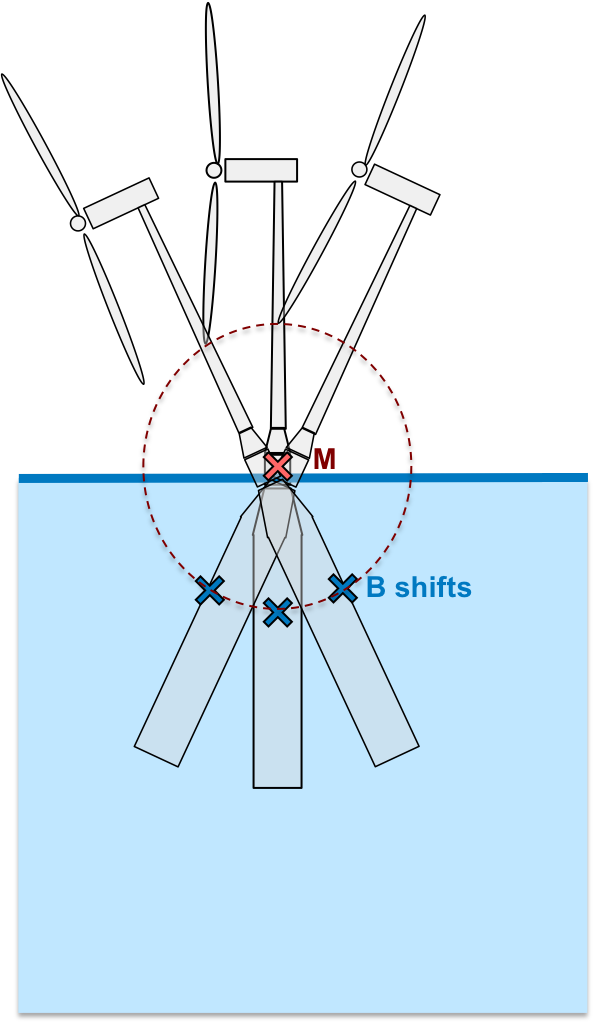
\includegraphics[height=3.5in]{figs/metacenterC}
    \caption{}
  \end{subfigure}
  \begin{subfigure}[b]{0.49\linewidth}
    \centering 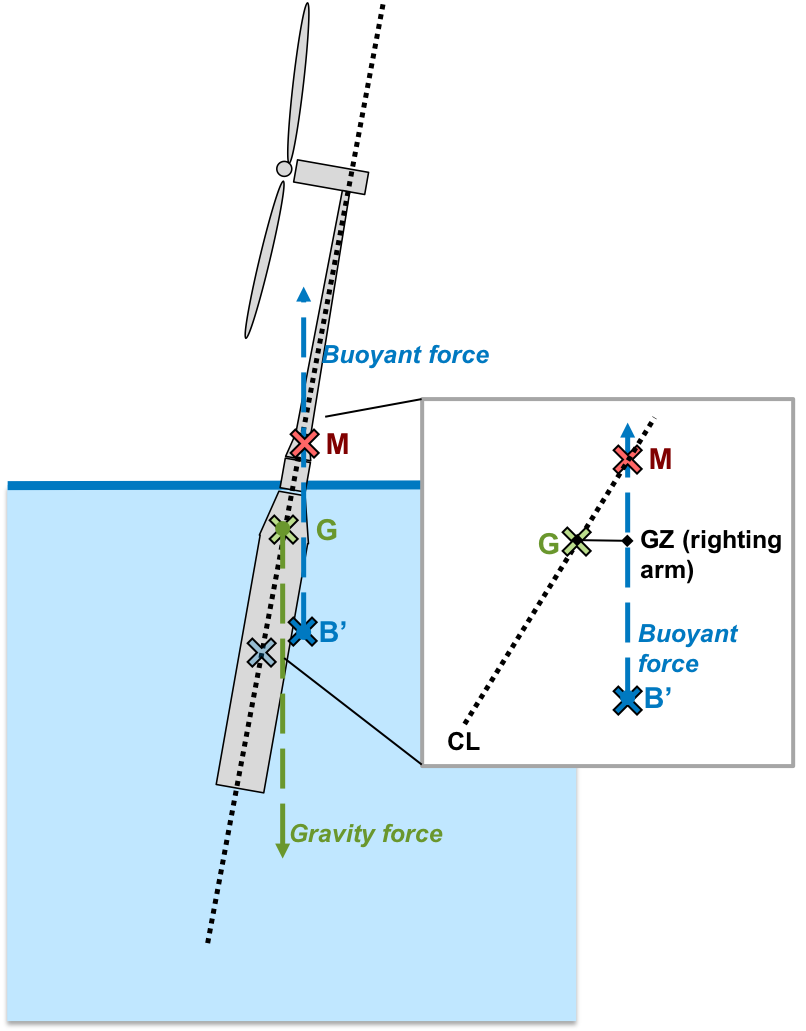
\includegraphics[height=3.5in]{figs/metacenterD}
    \caption{}
  \end{subfigure}
  \caption{Static stability of floating offshore wind turbines.}
  \label{fig:metacenter}
\end{figure}


The second contributing restoring moment comes from the motion of the
center of buoyancy away from alignment with the center of mass.  This is
a standard calculation in naval architecture \citep{thiagarajan2014} and is
diagrammed in Figure \ref{fig:metacenter}.  In this diagram, the center
of mass is denoted, $G$, the center of buoyancy is $B$, and the
metacenter is $M$.  In neural conditions (Figure \ref{fig:metacenter}a),
all of this points are vertically aligned.  The metacenter is defined as
the common point through which the buoyancy force acts as it pitches
through small displacements (Figure \ref{fig:metacenter}b--c), for bodies
with sufficient freeboard margin.  The metacenter point is most easily
calculated as an offset from the center of buoyancy ($BM$) by,
\[
  BM = \frac{I_w}{V}
\]
where $I_w$ is the second moment of area of the substructure waterplane
with units of \unit{$m^4$} and $V$ is the total volume of displacement
with units of \unit{$m^3$}.  Note that for semisubmersible type
geometries, $I_w$ is calculated with the parallel axis theorem for all
of the columns at the waterplane,
\[
  I_w = \sum_i \left( I_{w,i} + A_{w,i}r_i^2 \right)
\]
where $A_w$ is the cross sectional area of the $i$\th column and $r_i$
is the distance from the waterplane centroid to the $i$\th column centroid.

As the structure lists or heels, the center of buoyancy shifts toward
the side of the structure that is more submerged (from $B$ to $B'$) and
the buoyancy force no longer passes through the center of mass.
Instead, the buoyancy force passes through the metacenter (by its
definition) with an effective moment arm of $GZ$ from the center of mass
(Figure \ref{fig:metacenter}d).  By geometry,
\[
GZ = GM \sin \theta
\]
where $\theta$ is the angle of heel.  The restoring moment is then the
buoyancy force acting through the restoring arm, $GZ$,
\[
  M_{pitch} = F_B \left(GZ\right)
\]
For this reason, the metacenter must be located above the center of
mass for static stability.  This condition is imposed on the design as a
constraint.  Note that the total volume of displacement, and the
subsequent buoyancy force, is not recalculated in the perturbed
configuration.  It is assumed that the angles of deflection are small
and that there is sufficient freeboard and design symmetry such that the
total displacement is constant.

\subsubsection{Heave, Roll, Yaw Stability}
The heave, roll, and yaw degrees of freedom are not yet modeled in
\textit{FloatingSE}.  Future improvements to the module will consider adding
these features.

\subsection{Mooring Lines}
The steady-state mooring system analysis is handled by the external Mooring Analysis
Program (MAP++) library \citep{MAP}, which has convenient Python bindings
to access the simulation output.  From its website
(\url{https://nwtc.nrel.gov/MAP}),
\begin{quote}
  MAP is designed to be used in parallel with other tools to model the
  steady-state forces on a Multi-Segmented, Quasi-Static (MSQS) mooring
  line. The MSQS model is developed based on an extension of
  conventional single line static solutions. Conceptually, MAP++'s MSQS
  module solves the algebraic equations for all elements simultaneously
  with the condition that the total force at connection points sum to
  zero. Seabed contact, seabed friction, and externally applied forces
  can be modeled with this tool. This allows multi-element mooring lines
  with arbitrary connection configurations to be analyzed.
\end{quote}

MAP++ inputs are passed through a text-file, and include sea depth, geometry
descriptions of the mooring line connections, and material properties of
the lines.  For chain and rope-based cables, these material properties
are not easily derived and would be typically provided by a
manufacturer.  We borrow from the approach of the popular OrcaFlex
software \citet{orca} and use the following expressions,
\begin{align*}
MBL &= 2.74\times 10^7  D^2 \left(44 - 80D\right) \unit{N} \\
mass &= 19.9\times 10^3 D^2 \unit{kg/m}\\
A &= 2\left(\pi D^2 / 4 \right)\\
EA &= 0.854e11 D^2\unit{m^2}\\
cost &= 3.415\times 10^4 D^2 \unit{USD}
\end{align*}
where $MBL$ is minimum breaking load, $D$ is the diameter of a single
half-chain link, $A$ is the chain cross-sectional area, $E$ is the
Young's modulus, $EA$ is the axial stiffness.  When conducting
optimization, the expression for $MBL$ is poorly posed due to its limited
range of diameter applicability, so a linear fit is used instead,
\[
MBL = 1000 \max\left(1.0, -5445.3 + 176972.7 D\right)
\]  
